\Chapter{Megvalósítás}


\section{Adatbázisok és modellek}
A programban a drón, és telemetria adatmodell a legfontosabb. Ezeket az adatokat olvassuk és mentjük,
illetve szükségesek az azonosításhoz vagy bármilyen értelmes következtetéshez a problémához kapcsolódóan.

A programban a telemetria modell a következőképpen néz ki:
\begin{python}
    package models

    import "time"

    type Telemetry struct {
    Speed              int
    Location           GPS `json:"location"`
    Altitude           float64
    CompassDirection   float64
    Acceleration       float64
    BatteryLevel       int   `json:"battery_level"`
    BatteryTemperature int   `json:"battery_temperature"`
    MotorTemperatures  []int `json:"motor_temperatures"`
    TimeStamp          time.Time
    }

    type GPS struct {
    Latitude  float64 `json:"latitude"`
    Longitude float64 `json:"longitude"`
    }

\end{python}

\subsection{Relációs adatbázis, PostgreSQL modell}
A relációs adatbázissal is működik a szimuláció.
\paragraph{Relációs modell \ref{fig:postgres} } \mbox{} \\

\begin{figure}[h]
    \centering
    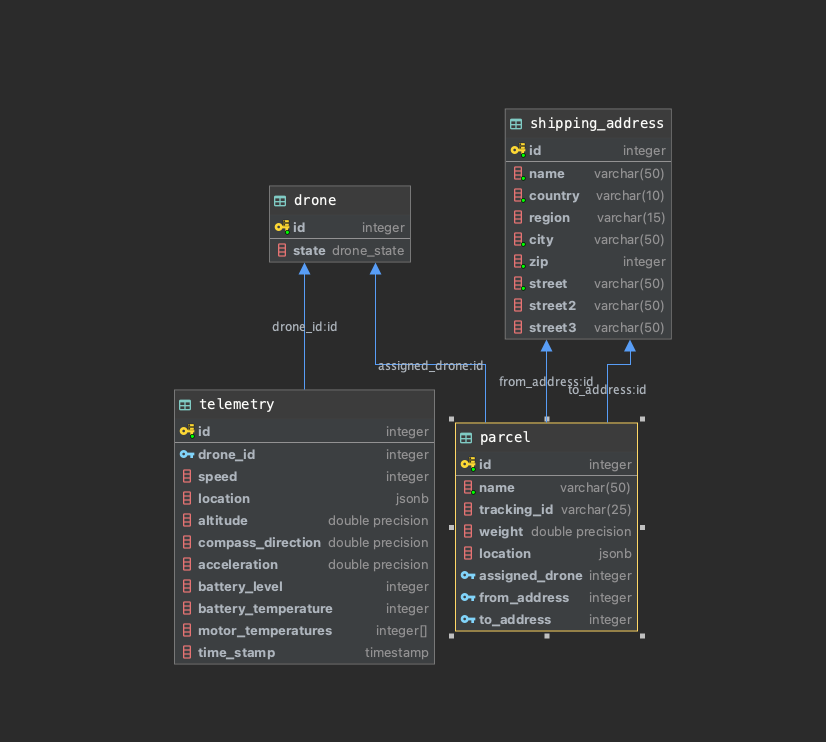
\includegraphics[scale=0.4]{images/postgres.png}
    \caption{PostgreSQL adatbázis modell}
    \label{fig:postgres}
\end{figure}

%TODO: ide táblázattal megcsinalni a relacios modellt

\paragraph{Lost Update probléma} \mbox{} \\
A legtöbb relációs adatbázis támogatja a tranzakciókat. A tranzakciók ACID tulajdonságokkal bírnak.
Adatbázisok esetén az ACID az Atomicity (atomiság), Consistency (konzisztencia), Isolation (izoláció), és Durability (tartósság) rövidítése. Ezek nélkül az adatbázis integritása nem garantálható.
A PostgreSQL többféle izolációs szintet biztosít a tranzakciókhoz \cite{postgres-transaction}. A Lost Update problémát garantáltan megoldja a PostgreSQL `Serializable` izolációs szintje.
\begin{table}[h]
    \centering
    \caption{ Standard SQL Transaction Isolation Levels}}
    \begin{tabular}{l|c|c|c|}
Isolation Level & Dirty Read  & Nonrepeatable Read & Phantom Read\\
        \hline
Read uncommitted  & Possible & Possible & Possible \\
\hline
Read committed & Not possible & Possible & Possible \\
\hline
Repeatable read & Not possible & Not possible & Possible \\
\hline
Serializable & Not possible & Not possible & Not Possible \\
        \hline
    \end{tabular}
\end{table}
